%%%% fs-run-mapreduce MapReduce transformation on stream

\label {fs-mapreduce}

In this section, we demonstrate a way of implementation of MapReduce-like transformation on a stream in order to show soundness of our model. Map stage of MapReduce is directly mapped on the map operation. However, it is not obvious how to implement reduce step, because it requires an explicit state handling. 

The pseudo-code of the classical MapReduce algorithm for word counting is shown on the figure <>. Map step of this algorithm transforms each input word into key-value pair where word is the key, and the value is 1. Reduce step sums all values into the final result for specific key. We can note, that there is a need to store and update current word count.

One possible way to implement reduce step in out model is to make business logic state a part of the stream, and work with it like with ordinary data item. Figure~\ref{mapreduce-graph-figure} shows a generic graph for MapReduce computation. Map and reduce parts are highlighted with dashed line.

\begin{figure}[htb]
  \centering
  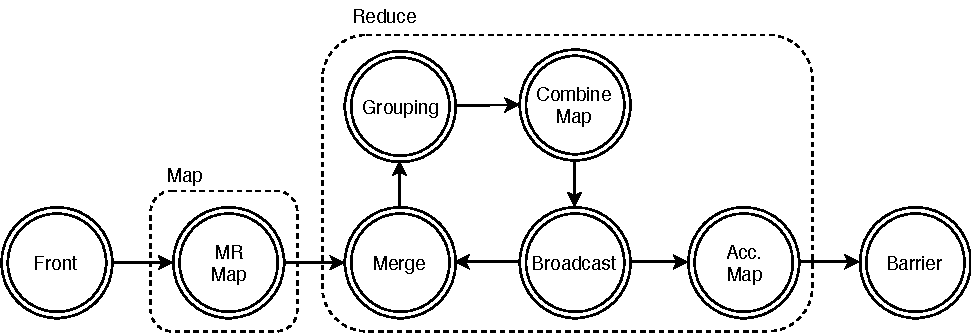
\includegraphics[scale=0.5]{pics/mapreduce}
  \caption{Logical graph for MapReduce transformations}
  \label {mapreduce-graph-figure}
\end{figure}

There are three types of data items in this stream: {\it input} items, {\it mapped} items, and {\it reduced} items. Each type of item and the way they were generated are detailed further in this section. However, it is worth to mention that mapped and reduced items have key-value structure of payload and presents intermediate values. The operations of the stream have the following purposes:

\begin{itemize}
\item The first map operation accepts input items and outputs mapped items according to map step of MapReduce model.
\item The window of grouping is set to 2. It is used to group current reduce state with next dataitem to combine them together further. The hash function is designed to return distinct values for payloads with distinct keys.
\item The second map implements the actual combining. Its input has a form of: \textit{(mapped item)} or \textit{(mapped item, reduced item)}. The first kind is transformed into some initial value. The second tuple is combined into reduce item as specified by reduce step of MapReduce. 
\item The intermediate filter operation removes tuples with structure \textit{(mapped item; reduced item)}, i.e. tuples, where mapped item is before reduced item so it was generated before reduced one.
\item Broadcast operation is used to return actual reduced item back to the grouping and, at the same time, to output it from stream. 
\end{itemize}

The key idea is that ordering assumptions about data items guarantees that each reduced item always arrives at grouping right after already combined mapped item and before a new one. Hence, each mapped item would be grouped with the actual reduced item. Additionally, when filter accepts tuple {\it (mapped item, reduced item)}, then it means that mapped item was generated before reduced, and therefore, it had been already combined. The cycle gives ability for new reduced items to get back in grouping operation. Thereby, the stream reacts to each input item by generating new reduced item, which contains the actual value of the reduce step.

\subsection{Word counting example}

The example of input/output items, which are generated/ transformed by the part of the logical graph, is shown on the figure~\ref {word-count-figure}. This example represents MapReduce-based algorithm for word counting, which was detailed above. According to our graph for MapReduce transformations, the item {\it m[dog, 1]} represents mapped item with key "dog" and value 1. The item {\it r[dog, 1]} describes reduced item with key "dog" and value 1. The figure shows how the model reacts on two consequent input items containing word "dog". The meta-information of items is omitted for simplification. More precisely, there are shown 4 stages separated by dotted lines:

\begin{enumerate}
    \item New mapped item with key "dog" arrives at grouping with empty state. Grouping outputs tuple with this single item. Filter accepts the tuple, and Map transforms it to the first reduced item for key "dog" and value 1.
    \item The reduced item arrives at grouping after it went through the cycle. It is grouped in tuple with mapped item that has been already in the state with key "dog". However, filter drops this tuple, because of the order of items.
    \item New mapped item with key "dog" arrives at grouping. It is inserted right after the reduced item in the bucket for key "dog". Grouping outputs tuple containing the reduced item and new mapped item. Filter accepts this tuple, because it has the right order. Map operation combines reduced and mapped items into new reduced items with key "dog" and value 2.
    \item New reduced item arrives at grouping through the cycle, but new generated tuple is not accepted by filter, as well as in the step 2.
\end{enumerate}

\begin{figure}[htb]
  \centering
  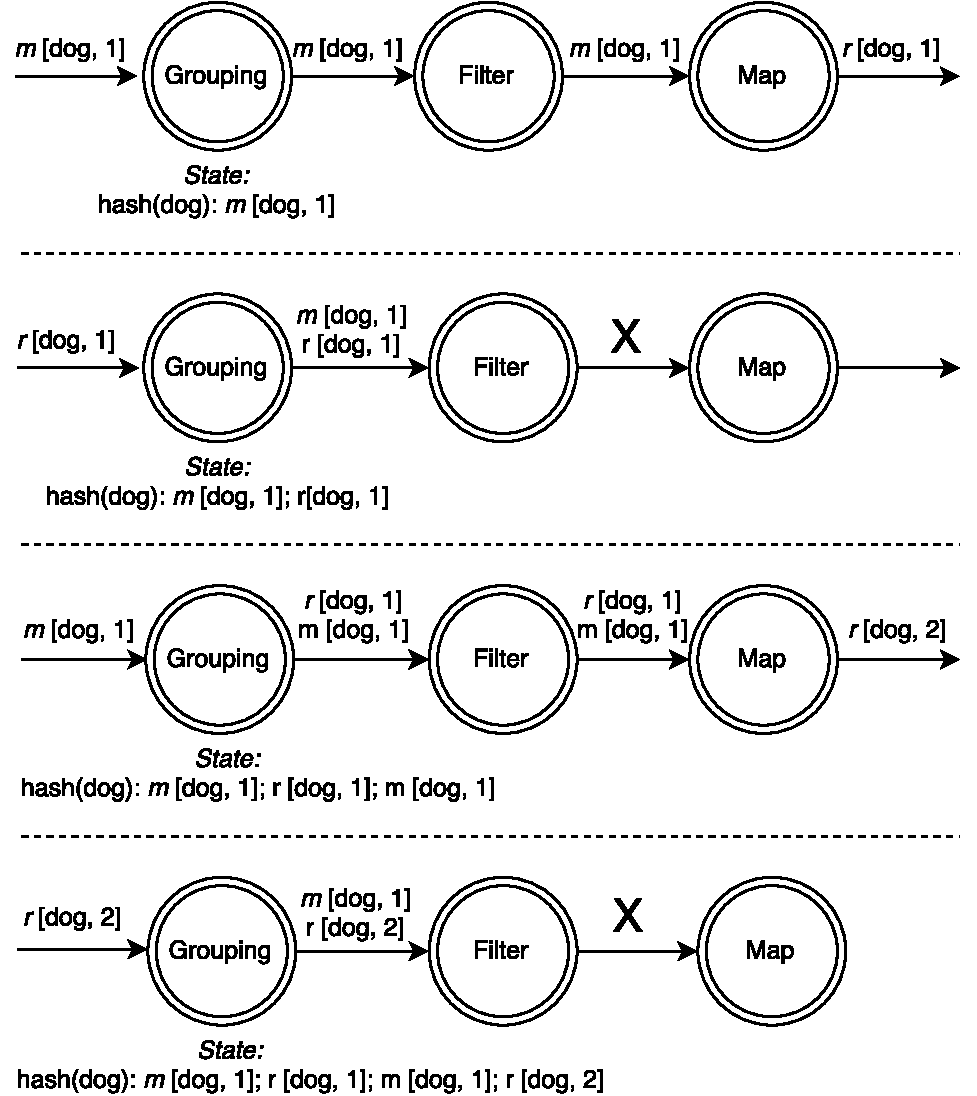
\includegraphics[scale=0.5]{pics/wordcount}
  \caption{Part of the stream evalutaion for word counting}
  \label {word-count-figure}
\end{figure}

